% =============================================================================
% Block 7 --- Aula 7: money and inflation (Kurlat chs. 10-11). Checks: practice-all-topics-check-b.py, Block 7.
% Solution format (rules/00_estilo_avaliacao.md §4): Notation list, numbered equations cited with \eqref,
% one operation per displayed line. Labels: b7q<question>:<name>.
\bloco{7}{Money and inflation: aggregates, money demand, the quantity theory, seigniorage}{Kurlat chs.~10--11 (Aula 7) \,\textbullet\, 25 points}

\questao{(5 points) Objective items.}

\textbf{a)} (3 points) A Brazilian saver holds a fixed-rate (\emph{prefixado}) bond. Income tax takes $\tau=15\%$ of the
\emph{nominal} interest. The real rate is $r=7\%$ and the Fisher effect holds ($i=r+\pi$). Anticipated inflation rises from
$5\%$ to $10\%$. The after-tax real return $(1-\tau)i-\pi$ goes:
\begin{alternativas}
\item from $5.95\%$ to $5.95\%$
\item from $5.2\%$ to $4.45\%$
\item from $7\%$ to $7\%$
\item from $12\%$ to $17\%$
\end{alternativas}
\gabarito{B}
\begin{sol}
\begin{notacao}
\item $i$: nominal rate; $r$: pre-tax real rate; $\pi$: anticipated inflation; $\tau\in(0,1)$: tax on nominal interest; $r^\tau$: after-tax real return.
\end{notacao}
\passo{computation}{The statement gives the Fisher relation and the after-tax real return:}
\begin{align}
i&=r+\pi, \label{b7q19:fisher}\\
r^\tau&=(1-\tau)i-\pi. \label{b7q19:ret}
\end{align}
Substituting \eqref{b7q19:fisher} into \eqref{b7q19:ret}:
\begin{align}
r^\tau&=(1-\tau)(r+\pi)-\pi\nonumber\\
&=(1-\tau)r-\tau\pi. \label{b7q19:ret2}
\end{align}
Before, by \eqref{b7q19:fisher} and then \eqref{b7q19:ret}; after, the same with $\pi=10$:
\begin{align*}
i&=7+5=12\%,\\
r^\tau&=(1-0.15)\times(12)-5\\
&=0.85\times12-5=10.2-5=5.2\%,\\
i&=7+10=17\%,\\
r^\tau&=(1-0.15)\times(17)-10\\
&=0.85\times17-10=14.45-10=4.45\%.
\end{align*}
By \eqref{b7q19:ret2}, the loss is $\tau\,\Delta\pi=0.15\times5=0.75$ points: the tax falls on the inflation premium, which is not income.
\passo{distractors}{A taxes only the real return, the first term of \eqref{b7q19:ret2}, $(1-\tau)r=0.85\times7=5.95\%$, as an indexed tax system would. C forgets the tax (the
Fisher effect alone keeps the pre-tax real rate at 7\%). D makes two mistakes: no tax and nominal instead of real returns.}
\refbib{Kurlat (2020), \S11.1 (Fisher equation) and \S11.4 (The Cost of Inflation), pp.~205--222.}
\end{sol}

\medskip
\textbf{b)} (2 points, T or F) With Baumol--Tobin money demand and flexible prices, a permanent, anticipated rise in the growth
rate of money raises inflation one for one in the new steady state and leaves real money balances unchanged.
\gabarito{F}
\begin{sol}
\begin{notacao}
\item $\mu$: money growth; $\pi$: inflation; $g$: real growth; $\eta$: income elasticity of money demand; $i$, $r$: nominal and
real rates; $M/P$: real balances; $F$: real cost of a bank trip; $Y$: real spending.
\end{notacao}
\passo{proof}{The first half is right: in a steady state}
\begin{equation}
\pi=\mu-\eta g, \label{b7q19:qt}
\end{equation}
with $g$ unchanged, so $d\pi=d\mu$. The second half is not. By Fisher, $i=r+\pi$, so $i$ rises one for one. Baumol--Tobin demand is
\begin{equation}
\frac MP=\sqrt{\frac{FY}{2i}}, \label{b7q19:bt}
\end{equation}
whose interest elasticity, from the log of \eqref{b7q19:bt}, is
\begin{equation}
\frac{\partial\ln(M/P)}{\partial\ln i}=-\frac12. \label{b7q19:el}
\end{equation}
By \eqref{b7q19:el}, real balances fall. Money is neutral in \emph{levels} but not superneutral:
a change in its \emph{growth rate} changes a real variable (and the resources spent on trips to the bank).
\refbib{Kurlat (2020), \S10.4 and \S11.2, pp.~199--215.}
\end{sol}

% -----------------------------------------------------------------------------
\questao{(8 points) \textit{Source: Kurlat, P. (2020), \emph{A Course in Modern Macroeconomics}, Exercise 11.6 ``Seignorage with High
Inflation'', pp.~219--221 --- reproduced verbatim; this list asks items (a)--(j) only (the book's items (k)--(u) are omitted).}}

\noindent Suppose that money demand is given by:
\[
m^D(Y_t,i_{t+1})=Y_t\cdot(1+i_{t+1})^{-\mu}
\]
where $\mu$ is a parameter. This is sometimes known as the Cagan money-demand function. Equilibrium in the money market is given by:
\[
M_t^S=Y_t\cdot(1+i_{t+1})^{-\mu}\,p_t
\]
The real economy is in a steady state so that:
\begin{align*}
Y_t&=Y_{ss}\\
r_{t+1}&=r_{ss}
\end{align*}
The government obtains seignorage revenue $S_t$ (in real terms) by expanding the monetary base. $S_t$ is given by:
\[
S_t=\frac{M_t^B-M_{t-1}^B}{P_t} \tag{11.4.2}
\]
Let $\omega$ be the money multiplier, so that $M^S=\omega M^B$.\par
\noindent Suppose that the rate of growth of the money supply is constant at rate $\gamma$, i.e.:
\[
M_t^S=(1+\gamma)\,M_{t-1}^S \tag{11.4.3}
\]
\begin{enumerate}[label=(\alph*),leftmargin=2.2em,topsep=2pt,itemsep=1pt]
\item What will be the rate of inflation?
\item What will be nominal interest rate?
\item Find an expression for the level of real money balances. How does it depend on $\gamma$? Why?
\item Solve equation (11.4.3) for $M_{t-1}^S$ and replace this in (11.4.2) to obtain an expression for seignorage revenue $S_t$ in terms
of $\gamma$ and $\frac{M_t^S}{P_t}$. How does $S_t$ depend on $\gamma$? How does it depend on $\frac{M_t^S}{P_t}$? Why?
\item Replace the value of $\frac{M_t^S}{P_t}$ that you found in part (c) into the expression for $S_t$ that you found in part (d) to
obtain an expression for seignorage revenues $S_t$ in terms of $\gamma$, $Y_{ss}$, $r_{ss}$, $\omega$ and $\mu$.
\item Assume the following parameter values:
\begin{align*}
Y_{ss}&=1\\
\mu&=4\\
r_{ss}&=0.0025\\
\omega&=5
\end{align*}
Note that $\mu=4$ is close to the value that has been empirically estimated in some high inflation countries when the time period
is one month. To be consistent, $r_{ss}$ should be interpreted as a monthly real interest rate and $Y_{ss}$ as monthly GDP.
\item Plot $S_t$ against $\gamma$ for values of $\gamma$ between 0 and 0.8.
\item What is the monthly rate of growth of the money supply that maximizes seignorage revenue? Call this $\gamma^*$.
\item Why is seignorage revenue decreasing in $\gamma$ for $\gamma>\gamma^*$?
\item What monthly inflation rate does $\gamma=\gamma^*$ imply?
\end{enumerate}
\noindent\textit{Added to the book's items (not in the book):} draw the plot of part (g). Careful with notation: here $\mu$ is the
Cagan semi-elasticity, not money growth ($\gamma$).
\resolespaco
\begin{sol}
\begin{notacao}
\item $M_t$: money (M1); $MB_t$: monetary base; $\omega>1$: money multiplier, $M_t=\omega MB_t$; $P_t$: price level.
\item $\gamma>0$: growth rate of money per month; $\pi$: inflation; $i$: nominal rate; $r_{ss}$: steady-state real rate.
\item $\mu>0$: Cagan semi-elasticity of money demand (\emph{not} money growth); $Y_{ss}$: steady-state real output.
\item $S_t$: real seignorage (revenue from issuing base money); $\gamma^\ast$: revenue-maximizing money growth.
\end{notacao}
\passo{(a) inflation}{In a steady state $Y_t=Y_{ss}$ and $r_{t+1}=r_{ss}$. Real money demand is}
\begin{equation}
\frac{M_t}{P_t}=Y_{ss}(1+i)^{-\mu}. \label{b7q20:md}
\end{equation}
If $\pi$ is constant, $i$ is constant, so by \eqref{b7q20:md} real balances are constant. Then prices grow with money:
\begin{equation}
\frac{P_t}{P_{t-1}}=\frac{M_t}{M_{t-1}}=1+\gamma, \label{b7q20:pi}
\end{equation}
so $\boxed{\pi=\gamma}$, consistent with the guess.
\passo{(b) nominal rate}{The exact Fisher equation is}
\begin{equation}
1+i=(1+r_{ss})(1+\pi). \label{b7q20:fisher}
\end{equation}
Using $\pi=\gamma$ from \eqref{b7q20:pi}:
\begin{equation}
1+i=(1+r_{ss})(1+\gamma), \label{b7q20:i}
\end{equation}
so $i=(1+r_{ss})(1+\gamma)-1\approx r_{ss}+\gamma$.
\passo{(c) real balances}{Substitute \eqref{b7q20:i} into \eqref{b7q20:md}:}
\begin{equation}
\frac{M_t}{P_t}=Y_{ss}\left[(1+r_{ss})(1+\gamma)\right]^{-\mu}, \label{b7q20:m}
\end{equation}
decreasing in $\gamma$: faster money growth means more inflation, a higher nominal rate and a higher cost of holding money, so
people hold less.
\passo{(d) seignorage}{The government issues only base money, and by \eqref{b7q20:pi} money grows at $\gamma$:}
\begin{align}
MB_t&=\frac{M_t}{\omega},\qquad M_{t-1}=\frac{M_t}{1+\gamma}, \label{b7q20:mb}\\
S_t&=\frac{MB_t-MB_{t-1}}{P_t}. \label{b7q20:Sdef}
\end{align}
Substitute \eqref{b7q20:mb} into \eqref{b7q20:Sdef}:
\begin{align}
S_t&=\frac{\big(\frac{M_t}{\omega}\big)-\big(\frac{M_t}{(1+\gamma)\,\omega}\big)}{P_t}\nonumber\\
&=\frac1\omega\,\frac{M_t-\frac{M_t}{1+\gamma}}{P_t}\nonumber\\
&=\frac{\gamma}{(1+\gamma)\,\omega}\,\frac{M_t}{P_t}. \label{b7q20:S}
\end{align}
Given $\frac MP$, $S$ rises with $\gamma$ (a higher tax rate) and is proportional to real balances (the tax base). It is divided by
$\omega$ because only base money is issued by the government; deposits created by banks are not its revenue.
\passo{(e) in parameters}{Substitute \eqref{b7q20:m} into \eqref{b7q20:S}:}
\begin{equation}
S=\frac{\gamma}{(1+\gamma)\,\omega}\,Y_{ss}\left[(1+r_{ss})(1+\gamma)\right]^{-\mu}. \label{b7q20:Sp}
\end{equation}
\passo{(f)--(g) plot}{With $Y_{ss}=1$, $\mu=4$, $r_{ss}=0.0025$, $\omega=5$, \eqref{b7q20:Sp} becomes}
\begin{align}
S(\gamma)&=\frac{\gamma}{(1+\gamma)\,(5)}\,(1)\left[(1+0.0025)(1+\gamma)\right]^{-(4)}\nonumber\\
&=\frac{\gamma}{5(1+\gamma)}\left[1.0025(1+\gamma)\right]^{-4}. \label{b7q20:Snum}
\end{align}
\begin{center}
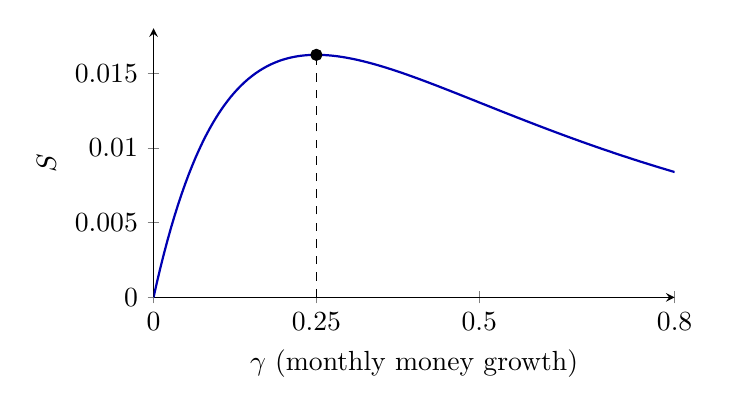
\begin{tikzpicture}
\begin{axis}[width=8.2cm,height=5cm,xmin=0,xmax=0.8,ymin=0,ymax=0.018,xlabel={$\gamma$ (monthly money growth)},ylabel={$S$},
  axis lines=left,scaled y ticks=false,yticklabel style={/pgf/number format/fixed,/pgf/number format/precision=3},
  xtick={0,0.25,0.5,0.8}]
\addplot[blue!70!black,thick,domain=0:0.8,samples=150] {x/(5*(1+x))*(1.0025*(1+x))^(-4)};
\addplot[dashed] coordinates {(0.25,0) (0.25,0.01622)};
\addplot[only marks,mark=*] coordinates {(0.25,0.01622)};
\end{axis}
\end{tikzpicture}
\end{center}
It rises from $0$, peaks at $\gamma=0.25$ ($S=0.0162$) and falls to $0.0084$ at $\gamma=0.8$: a Laffer curve.
\passo{(h) maximum}{Take the log of \eqref{b7q20:Sp}:}
\begin{equation}
\ln S=\ln\gamma-\ln(1+\gamma)-\ln\omega+\ln Y_{ss}-\mu\ln(1+r_{ss})-\mu\ln(1+\gamma). \label{b7q20:lnS}
\end{equation}
Differentiate \eqref{b7q20:lnS} with respect to $\gamma$:
\begin{align}
\frac{d\ln S}{d\gamma}&=\frac1\gamma-\frac{1}{1+\gamma}-\frac{\mu}{1+\gamma}\nonumber\\
&=\frac1\gamma-\frac{1+\mu}{1+\gamma}\nonumber\\
&=\frac{1-\mu\gamma}{\gamma(1+\gamma)}. \label{b7q20:dlnS}
\end{align}
\eqref{b7q20:dlnS} is zero at $\boxed{\gamma^\ast=1/\mu=0.25}$ per month; positive below, negative above, so it is the maximum.
Revenue there, from \eqref{b7q20:Snum}:
\begin{align*}
S^\ast&=\frac{0.25}{5(1+0.25)}\left[1.0025(1+0.25)\right]^{-4},\\
1.0025\times1.25&=1.253125,\\
1.253125^4&=2.4659,\\
S^\ast&=\frac{0.25}{5\times1.25}\cdot\frac1{2.4659}=\frac{0.04}{2.4659}=0.0162,
\end{align*}
about $1.6\%$ of monthly GDP, with real balances $1/2.4659=0.4055$ by \eqref{b7q20:m} and $i=25.3\%$ a month by \eqref{b7q20:i}.
\passo{(i) why it falls}{The first line of \eqref{b7q20:dlnS} adds the gain in the rate, $\frac1\gamma-\frac1{1+\gamma}=\frac1{\gamma(1+\gamma)}$, and the loss in the base, $-\frac{\mu}{1+\gamma}$.
For $\gamma>1/\mu$ the base shrinks faster than the rate rises: people economize so much on money that more inflation collects less.}
\passo{(j) inflation}{By \eqref{b7q20:pi}, $\pi=\gamma^\ast=25\%$ a month, i.e.\ $1.25^{12}-1=13.55$, about $1{,}355\%$ a year: a high-inflation regime of the
kind Brazil lived through before the Plano Real.}
\intuicao{Seignorage is a tax whose base is the public's real balances; the base responds to the rate through the Cagan
semi-elasticity $\mu$, so the revenue-maximizing money growth is $1/\mu$, and governments that print faster collect less.}
\refbib{Kurlat (2020), \S11.3 (Seignorage), eq.~(11.4.2), pp.~215--218; Exercise 11.6, pp.~219--220. Same result
($\pi^{\max}=1/a$ in the continuous Cagan form) in the project's Map notes (Aula 7, note 04, \S4.2). No instructor key covers 11.6.}
\rubrica{
\item (a)--(c) 2 pts; (d)--(e) 2 pts; (f)--(g) plot with labeled axes and the peak marked 1 pt; (h) 2 pts (FOC 1, $\gamma^\ast$ and $S^\ast$ 1); (i)--(j) 1 pt.
\item Seignorage written as $\pi\frac MP$ without the base/multiplier step: max.\ 1 pt in (d)--(e). Treating more money growth as always more revenue: 0 in (i).
}
\end{sol}

% -----------------------------------------------------------------------------
\questao{(12 points) Discursive. \emph{From the monetary base to the price level: a credible disinflation.} The Banco Central do
Brasil (BCB) controls the base $B$. The public holds currency and deposits in the ratio $c=C/D=0.25$; banks hold reserves (required
plus excess) in the ratio $\theta=R/D=0.20$. Real money demand follows Baumol--Tobin: spending $Y$ per period is withdrawn in
$N$ equal trips to the bank, each costing $F$ in real terms. Prices are flexible, real output grows at $g=2\%$, the real rate is
constant at $r=4\%$ and M1 grows at $\mu=6\%$ (illustrative values).}

\textbf{a)} (3 points) Derive the money multiplier $m=M1/B$ and compute it. The BCB cuts reserve requirements so that $\theta$ falls to
$0.15$: by how much does M1 change for a given base? Why is $m$ not a constant the BCB can rely on?
\resolespaco
\begin{sol}
\begin{notacao}
\item $B$: monetary base; $C$: currency held by the public; $D$: deposits; $R$: bank reserves; $M1$: currency plus deposits.
\item $c=C/D>0$: currency-deposit ratio; $\theta=R/D\in(0,1)$: reserve ratio; $m=M1/B$: money multiplier.
\end{notacao}
\passo{derivation}{The two identities are}
\begin{align}
B&=C+R, \label{b7q21:B}\\
M1&=C+D. \label{b7q21:M1}
\end{align}
Divide \eqref{b7q21:B} and \eqref{b7q21:M1} by $D$:
\begin{align}
\frac BD&=c+\theta, \label{b7q21:BD}\\
\frac{M1}D&=1+c. \label{b7q21:MD}
\end{align}
Divide \eqref{b7q21:MD} by \eqref{b7q21:BD}:
\begin{equation}
m=\frac{M1}{B}=\frac{1+c}{c+\theta}. \label{b7q21:m}
\end{equation}
\passo{numbers}{From \eqref{b7q21:m}:}
\begin{align*}
m_0&=\frac{1+0.25}{0.25+0.20}\\
&=\frac{1.25}{0.45}=2.778,\\
m_1&=\frac{1+0.25}{0.25+0.15}\\
&=\frac{1.25}{0.40}=3.125,\\
\frac{m_1}{m_0}&=\frac{(1.25/0.40)}{(1.25/0.45)}\\
&=\frac{0.45}{0.40}=1.125 .
\end{align*}
M1 rises by $12.5\%$ with the same base; differentiating \eqref{b7q21:m}, $\partial m/\partial\theta=-\frac{1+c}{(c+\theta)^2}<0$.
\passo{caveat}{\eqref{b7q21:m} is an identity in two behavioral ratios. Banks choose excess reserves and the public chooses $c$; in a crisis both rise
and $m$ collapses (as in 2008), so a given base does not pin down M1.}
\rubrica{\item Derivation 1 pt; numbers 1 pt; why $m$ moves 1 pt.}
\end{sol}

\textbf{b)} (3 points) Derive Baumol--Tobin money demand, its income and interest elasticities, and the implied velocity.
\resolespaco
\begin{sol}
\begin{notacao}
\item $Y>0$: real spending per period; $N>0$: trips to the bank per period; $F>0$: real cost of a trip; $i>0$: nominal rate.
\item $\mathcal C(N)$: total cost of managing cash; $\ell\equiv M/P$: real money balances; $V$: velocity; $P$: price level.
\end{notacao}
\passo{problem}{With $N$ trips, cash falls from $Y/N$ to 0 between trips, so average real balances are}
\begin{equation}
\ell=\frac{Y}{2N}. \label{b7q21:avg}
\end{equation}
The total cost is trips plus the interest forgone on \eqref{b7q21:avg}:
\begin{equation}
\mathcal C(N)=FN+i\,\frac{Y}{2N}. \label{b7q21:cost}
\end{equation}
Differentiate \eqref{b7q21:cost} and set it to zero:
\begin{equation}
F-\frac{iY}{2N^2}=0. \label{b7q21:foc}
\end{equation}
Solve \eqref{b7q21:foc} for $N$ (the second derivative is $\frac{iY}{N^3}>0$, so it is a minimum):
\begin{equation}
N^\ast=\sqrt{\frac{iY}{2F}}. \label{b7q21:N}
\end{equation}
\passo{demand}{Substitute \eqref{b7q21:N} into \eqref{b7q21:avg}:}
\begin{align}
\ell&=\frac{Y}{2\Big(\sqrt{\frac{iY}{2F}}\Big)}\nonumber\\
&=\frac Y2\sqrt{\frac{2F}{iY}}\nonumber\\
&=\sqrt{\frac{FY}{2i}}. \label{b7q21:bt}
\end{align}
Taking logs of \eqref{b7q21:bt}, $\ln\ell=\frac12(\ln F+\ln Y-\ln2-\ln i)$, so
\[
\frac{\partial\ln\ell}{\partial\ln Y}=\frac12,\qquad \frac{\partial\ln\ell}{\partial\ln i}=-\frac12 .
\]
\passo{velocity}{The quantity equation is}
\begin{equation}
MV=PY. \label{b7q21:qt}
\end{equation}
Solve \eqref{b7q21:qt} for $V$ and use \eqref{b7q21:bt}:
\begin{align}
V&=\frac{Y}{\ell}=\frac{Y}{\sqrt{FY/(2i)}}\nonumber\\
&=\sqrt{\frac{2iY}{F}}. \label{b7q21:V}
\end{align}
It rises with $i$ and $Y$ and falls with $F$. So $V$ is not a constant and \eqref{b7q21:qt}, an identity, becomes a theory only once
$V$ is pinned down by a money-demand function.
\rubrica{\item Cost function and FOC: 1 pt. \item Demand and both elasticities: 1 pt. \item Velocity and the identity remark: 1 pt.}
\end{sol}

\textbf{c)} (3 points) In a steady state with constant $i$, show that $\pi=\mu-\eta g$, where $\eta$ is the income elasticity of money
demand. Compute $\pi$ and $i$ (exact Fisher) now, and the money growth the BCB needs for an inflation target of $3\%$.
\resolespaco
\begin{sol}
\begin{notacao}
\item $M$: M1; $\ell^D(Y,i)$: real money demand; $\mu=\dot M/M$: growth of M1; $\pi=\dot P/P$: inflation; $g=\dot Y/Y$: real growth.
\item $\eta\equiv\frac{\partial\ell^D}{\partial Y}\frac{Y}{\ell^D}$: income elasticity of money demand; $r$: real rate; $i$: nominal rate.
\end{notacao}
\passo{derivation}{In equilibrium money supply equals money demand:}
\begin{equation}
M=P\,\ell^D(Y,i). \label{b7q21:eq}
\end{equation}
Log-differentiate \eqref{b7q21:eq} in time, with $\dot i=0$:
\begin{equation}
\frac{\dot M}M=\frac{\dot P}P+\frac{\partial\ell^D}{\partial Y}\frac{Y}{\ell^D}\frac{\dot Y}Y. \label{b7q21:logd}
\end{equation}
In the notation above, \eqref{b7q21:logd} reads $\mu=\pi+\eta g$, so
\begin{equation}
\pi=\mu-\eta g. \label{b7q21:pi}
\end{equation}
Baumol--Tobin \eqref{b7q21:bt} gives $\eta=\frac12$.
\passo{numbers}{By \eqref{b7q21:pi}, $\pi_0=6-\frac12\times2=5\%$. The exact Fisher equation is}
\begin{equation}
1+i=(1+r)(1+\pi). \label{b7q21:fisher}
\end{equation}
By \eqref{b7q21:fisher}, $1+i_0=1.04\times1.05=1.092$, so $i_0=9.2\%$ (approximate: $9\%$). For the target $\pi_1=3\%$, solve \eqref{b7q21:pi} for $\mu$:
\begin{align*}
\mu_1&=\pi_1+\eta g\\
&=3+\tfrac12\times2=4\%,\\
1+i_1&=1.04\times1.03=1.0712,\quad i_1=7.12\%.
\end{align*}
\refbib{Instructor's key, PSET~6 Q2(a)--(b) (Lista~6): same derivation and $\eta=\tfrac12$, $\mu=3.5\%$ for a $2\%$ target with $g=3\%$.}
\rubrica{\item Derivation with $\dot i=0$ stated: 1.5 pts. \item Numbers: 1.5 pts. Using $\pi=\mu-g$ ($\eta=1$) for Baumol--Tobin: max.\ 1 pt.}
\end{sol}

\textbf{d)} (3 points) At date $T$ the BCB announces, credibly, that M1 will grow at $4\%$ from now on; $M_T$ itself does not change.
What happens to the price level at $T$ and afterwards? Draw $\ln P_t$. Is money superneutral here? What one-off operation would
avoid any jump in $P$?
\resolespaco
\begin{sol}
\begin{notacao}
\item $T$: announcement date; $M_T$: M1 at $T$ (given); $P_T$: price level at $T$.
\item $\ell_0,\ell_1$: desired real balances under the old ($i_0$) and new ($i_1$) steady states, at the same $Y_T$, $F$.
\end{notacao}
\passo{real balances}{By \eqref{b7q21:bt}, with $F$ and $Y_T$ the same in both regimes, desired balances scale with $i^{-1/2}$. Using $i_0$, $i_1$ from (c):}
\begin{align}
\frac{\ell_1}{\ell_0}&=\frac{\big(\sqrt{FY_T/(2i_1)}\big)}{\big(\sqrt{FY_T/(2i_0)}\big)}\nonumber\\
&=\sqrt{\frac{i_0}{i_1}} \label{b7q21:ratio}\\
&=\sqrt{\frac{0.092}{0.0712}}=\sqrt{1.2921}=1.1367.\nonumber
\end{align}
\passo{the jump}{The money market clears at $T$ with $M_T$ given, so by \eqref{b7q21:eq}}
\begin{equation}
P_T=\frac{M_T}{\ell}. \label{b7q21:PT}
\end{equation}
Dividing \eqref{b7q21:PT} under the new and old demand, then using \eqref{b7q21:ratio}:
\begin{align*}
\frac{P_T^{\text{new}}}{P_T^{\text{old}}}&=\frac{(M_T/\ell_1)}{(M_T/\ell_0)}\\
&=\frac{\ell_0}{\ell_1}=\frac1{(1.1367)}.
\end{align*}
$P$ falls by $12.0\%$ at $T$ ($\Delta\ln P=-\frac12\ln1.2921=-0.128$), then by \eqref{b7q21:pi} grows at $3\%$ instead of $5\%$.
\begin{center}
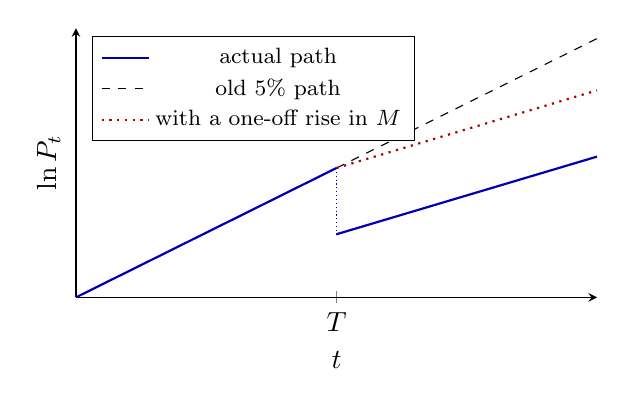
\begin{tikzpicture}
\begin{axis}[width=8.2cm,height=5cm,xmin=0,xmax=10,ymin=0,ymax=0.52,xlabel={$t$},ylabel={$\ln P_t$},axis lines=left,
  xtick={5},xticklabels={$T$},ytick=\empty,legend pos=north west,legend style={font=\footnotesize}]
\addplot[blue!70!black,thick] coordinates {(0,0) (5,0.25)}; \addlegendentry{actual path}
\addplot[black,dashed] coordinates {(5,0.25) (10,0.5)}; \addlegendentry{old $5\%$ path}
\addplot[red!70!black,dotted,thick] coordinates {(5,0.25) (10,0.40)}; \addlegendentry{with a one-off rise in $M$}
\addplot[blue!70!black,thick,forget plot] coordinates {(5,0.122) (10,0.272)};
\addplot[blue!70!black,densely dotted,forget plot] coordinates {(5,0.25) (5,0.122)};
\end{axis}
\end{tikzpicture}
\end{center}
\passo{superneutrality}{No: by \eqref{b7q21:ratio}, a change in money \emph{growth} changed real balances by $13.7\%$ (and the resources spent on bank trips).
Money is neutral only in \emph{levels}.}
\passo{avoiding the jump}{By \eqref{b7q21:PT}, $P_T$ is unchanged if $M_T$ rises in the same proportion as $\ell$. So raise $M$ once at $T$ by $13.7\%$
(buy bonds, expanding the base) and let it grow at $4\%$ afterwards: the public's higher demand for real balances is met by more
money instead of a lower $P$ (the remonetization seen in Brazil after the Plano Real).}
\intuicao{Lower expected inflation lowers the cost of holding money, so the public wants more of it at once; with $M$ fixed the only
way to supply real balances is a fall in $P$.}
\refbib{Kurlat (2020), \S11.2 (steady states with money growth), pp.~208--215; project Map notes (Aula 7, note 03, \S3.6).}
\rubrica{\item Ratio of real balances 1 pt. \item Jump with sign and size, graph with axes and slopes: 1 pt (graph alone 0.5).
\item Superneutrality and the one-off injection: 1 pt. A jump \emph{up} in $P$: max.\ 1 pt in the item.}
\end{sol}
